%\subsection{Portfolio f\"ur Research Object und Property Instance (Gr\"o\ss{}e entspricht der Anzahl)}
%\begin{figure}
\begin{center}
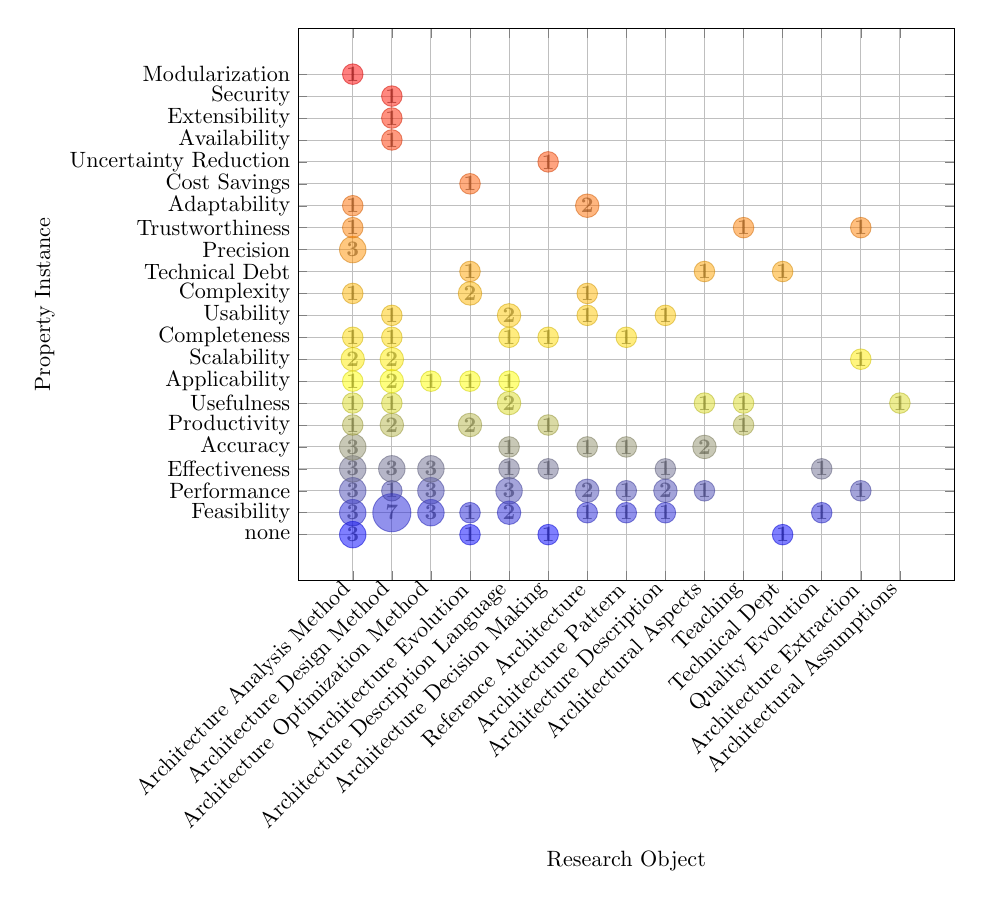
\begin{tikzpicture}[scale=.8]
\begin{axis}[scatter,
    width=.99\linewidth,
    cycle multi list=Spectral,
    every axis plot/.append style={draw, fill, fill opacity=0.5},
    scatter src=y,
    nodes near coords style={color=black,font=\small},
    %enlargelimits=0.15,
    x tick label style={rotate=45,anchor=east},
    xtick={0,1,2,3,4,5,6,7,8,9,10,11,12,13,14}, xticklabels={Architecture Analysis Method,Architecture Design Method,Architecture Optimization Method,Architecture Evolution,Architecture Description Language,Architecture Decision Making,Reference Architecture,Architecture Pattern,Architecture Description,Architectural Aspects,Teaching,Technical Dept,Quality Evolution,Architecture Extraction,Architectural Assumptions},
    xlabel={Research Object},
    ytick={0,1,2,3,4,5,6,7,8,9,10,11,12,13,14,15,16,17,18,19,20,21}, yticklabels={none,Feasibility,Performance,Effectiveness,Accuracy,Productivity,Usefulness,Applicability,Scalability,Completeness,Usability,Complexity,Technical Debt,Precision,Trustworthiness,Adaptability,Cost Savings,Uncertainty Reduction,Availability,Extensibility,Security,Modularization},
    ylabel={Property Instance},
    grid=both
]

\addplot[mark size=5.983,opacity=0.5,text=black] coordinates { (0,0) } node[text=black,font=\bfseries] {3};
\addplot[mark size=5.983,opacity=0.5,text=black] coordinates { (0,1) } node[text=black,font=\bfseries] {3};
\addplot[mark size=5.983,opacity=0.5,text=black] coordinates { (0,2) } node[text=black,font=\bfseries] {3};
\addplot[mark size=5.983,opacity=0.5,text=black] coordinates { (0,3) } node[text=black,font=\bfseries] {3};
\addplot[mark size=5.983,opacity=0.5,text=black] coordinates { (0,4) } node[text=black,font=\bfseries] {3};
\addplot[mark size=4.661,opacity=0.5,text=black] coordinates { (0,5) } node[text=black,font=\bfseries] {1};
\addplot[mark size=4.661,opacity=0.5,text=black] coordinates { (0,6) } node[text=black,font=\bfseries] {1};
\addplot[mark size=4.661,opacity=0.5,text=black] coordinates { (0,7) } node[text=black,font=\bfseries] {1};
\addplot[mark size=5.322,opacity=0.5,text=black] coordinates { (0,8) } node[text=black,font=\bfseries] {2};
\addplot[mark size=4.661,opacity=0.5,text=black] coordinates { (0,9) } node[text=black,font=\bfseries] {1};
\addplot[mark size=4.661,opacity=0.5,text=black] coordinates { (0,11) } node[text=black,font=\bfseries] {1};
\addplot[mark size=5.983,opacity=0.5,text=black] coordinates { (0,13) } node[text=black,font=\bfseries] {3};
\addplot[mark size=4.661,opacity=0.5,text=black] coordinates { (0,14) } node[text=black,font=\bfseries] {1};
\addplot[mark size=4.661,opacity=0.5,text=black] coordinates { (0,15) } node[text=black,font=\bfseries] {1};
\addplot[mark size=4.661,opacity=0.5,text=black] coordinates { (0,21) } node[text=black,font=\bfseries] {1};
\addplot[mark size=8.628,opacity=0.5,text=black] coordinates { (1,1) } node[text=black,font=\bfseries] {7};
\addplot[mark size=4.661,opacity=0.5,text=black] coordinates { (1,2) } node[text=black,font=\bfseries] {1};
\addplot[mark size=5.983,opacity=0.5,text=black] coordinates { (1,3) } node[text=black,font=\bfseries] {3};
\addplot[mark size=5.322,opacity=0.5,text=black] coordinates { (1,5) } node[text=black,font=\bfseries] {2};
\addplot[mark size=4.661,opacity=0.5,text=black] coordinates { (1,6) } node[text=black,font=\bfseries] {1};
\addplot[mark size=5.322,opacity=0.5,text=black] coordinates { (1,7) } node[text=black,font=\bfseries] {2};
\addplot[mark size=5.322,opacity=0.5,text=black] coordinates { (1,8) } node[text=black,font=\bfseries] {2};
\addplot[mark size=4.661,opacity=0.5,text=black] coordinates { (1,9) } node[text=black,font=\bfseries] {1};
\addplot[mark size=4.661,opacity=0.5,text=black] coordinates { (1,10) } node[text=black,font=\bfseries] {1};
\addplot[mark size=4.661,opacity=0.5,text=black] coordinates { (1,18) } node[text=black,font=\bfseries] {1};
\addplot[mark size=4.661,opacity=0.5,text=black] coordinates { (1,19) } node[text=black,font=\bfseries] {1};
\addplot[mark size=4.661,opacity=0.5,text=black] coordinates { (1,20) } node[text=black,font=\bfseries] {1};
\addplot[mark size=5.983,opacity=0.5,text=black] coordinates { (2,1) } node[text=black,font=\bfseries] {3};
\addplot[mark size=5.983,opacity=0.5,text=black] coordinates { (2,2) } node[text=black,font=\bfseries] {3};
\addplot[mark size=5.983,opacity=0.5,text=black] coordinates { (2,3) } node[text=black,font=\bfseries] {3};
\addplot[mark size=4.661,opacity=0.5,text=black] coordinates { (2,7) } node[text=black,font=\bfseries] {1};
\addplot[mark size=4.661,opacity=0.5,text=black] coordinates { (3,0) } node[text=black,font=\bfseries] {1};
\addplot[mark size=4.661,opacity=0.5,text=black] coordinates { (3,1) } node[text=black,font=\bfseries] {1};
\addplot[mark size=5.322,opacity=0.5,text=black] coordinates { (3,5) } node[text=black,font=\bfseries] {2};
\addplot[mark size=4.661,opacity=0.5,text=black] coordinates { (3,7) } node[text=black,font=\bfseries] {1};
\addplot[mark size=5.322,opacity=0.5,text=black] coordinates { (3,11) } node[text=black,font=\bfseries] {2};
\addplot[mark size=4.661,opacity=0.5,text=black] coordinates { (3,12) } node[text=black,font=\bfseries] {1};
\addplot[mark size=4.661,opacity=0.5,text=black] coordinates { (3,16) } node[text=black,font=\bfseries] {1};
\addplot[mark size=5.322,opacity=0.5,text=black] coordinates { (4,1) } node[text=black,font=\bfseries] {2};
\addplot[mark size=5.983,opacity=0.5,text=black] coordinates { (4,2) } node[text=black,font=\bfseries] {3};
\addplot[mark size=4.661,opacity=0.5,text=black] coordinates { (4,3) } node[text=black,font=\bfseries] {1};
\addplot[mark size=4.661,opacity=0.5,text=black] coordinates { (4,4) } node[text=black,font=\bfseries] {1};
\addplot[mark size=5.322,opacity=0.5,text=black] coordinates { (4,6) } node[text=black,font=\bfseries] {2};
\addplot[mark size=4.661,opacity=0.5,text=black] coordinates { (4,7) } node[text=black,font=\bfseries] {1};
\addplot[mark size=4.661,opacity=0.5,text=black] coordinates { (4,9) } node[text=black,font=\bfseries] {1};
\addplot[mark size=5.322,opacity=0.5,text=black] coordinates { (4,10) } node[text=black,font=\bfseries] {2};
\addplot[mark size=4.661,opacity=0.5,text=black] coordinates { (5,0) } node[text=black,font=\bfseries] {1};
\addplot[mark size=4.661,opacity=0.5,text=black] coordinates { (5,3) } node[text=black,font=\bfseries] {1};
\addplot[mark size=4.661,opacity=0.5,text=black] coordinates { (5,5) } node[text=black,font=\bfseries] {1};
\addplot[mark size=4.661,opacity=0.5,text=black] coordinates { (5,9) } node[text=black,font=\bfseries] {1};
\addplot[mark size=4.661,opacity=0.5,text=black] coordinates { (5,17) } node[text=black,font=\bfseries] {1};
\addplot[mark size=4.661,opacity=0.5,text=black] coordinates { (6,1) } node[text=black,font=\bfseries] {1};
\addplot[mark size=5.322,opacity=0.5,text=black] coordinates { (6,2) } node[text=black,font=\bfseries] {2};
\addplot[mark size=4.661,opacity=0.5,text=black] coordinates { (6,4) } node[text=black,font=\bfseries] {1};
\addplot[mark size=4.661,opacity=0.5,text=black] coordinates { (6,10) } node[text=black,font=\bfseries] {1};
\addplot[mark size=4.661,opacity=0.5,text=black] coordinates { (6,11) } node[text=black,font=\bfseries] {1};
\addplot[mark size=5.322,opacity=0.5,text=black] coordinates { (6,15) } node[text=black,font=\bfseries] {2};
\addplot[mark size=4.661,opacity=0.5,text=black] coordinates { (7,1) } node[text=black,font=\bfseries] {1};
\addplot[mark size=4.661,opacity=0.5,text=black] coordinates { (7,2) } node[text=black,font=\bfseries] {1};
\addplot[mark size=4.661,opacity=0.5,text=black] coordinates { (7,4) } node[text=black,font=\bfseries] {1};
\addplot[mark size=4.661,opacity=0.5,text=black] coordinates { (7,9) } node[text=black,font=\bfseries] {1};
\addplot[mark size=4.661,opacity=0.5,text=black] coordinates { (8,1) } node[text=black,font=\bfseries] {1};
\addplot[mark size=5.322,opacity=0.5,text=black] coordinates { (8,2) } node[text=black,font=\bfseries] {2};
\addplot[mark size=4.661,opacity=0.5,text=black] coordinates { (8,3) } node[text=black,font=\bfseries] {1};
\addplot[mark size=4.661,opacity=0.5,text=black] coordinates { (8,10) } node[text=black,font=\bfseries] {1};
\addplot[mark size=4.661,opacity=0.5,text=black] coordinates { (9,2) } node[text=black,font=\bfseries] {1};
\addplot[mark size=5.322,opacity=0.5,text=black] coordinates { (9,4) } node[text=black,font=\bfseries] {2};
\addplot[mark size=4.661,opacity=0.5,text=black] coordinates { (9,6) } node[text=black,font=\bfseries] {1};
\addplot[mark size=4.661,opacity=0.5,text=black] coordinates { (9,12) } node[text=black,font=\bfseries] {1};
\addplot[mark size=4.661,opacity=0.5,text=black] coordinates { (10,5) } node[text=black,font=\bfseries] {1};
\addplot[mark size=4.661,opacity=0.5,text=black] coordinates { (10,6) } node[text=black,font=\bfseries] {1};
\addplot[mark size=4.661,opacity=0.5,text=black] coordinates { (10,14) } node[text=black,font=\bfseries] {1};
\addplot[mark size=4.661,opacity=0.5,text=black] coordinates { (11,0) } node[text=black,font=\bfseries] {1};
\addplot[mark size=4.661,opacity=0.5,text=black] coordinates { (11,12) } node[text=black,font=\bfseries] {1};
\addplot[mark size=4.661,opacity=0.5,text=black] coordinates { (12,1) } node[text=black,font=\bfseries] {1};
\addplot[mark size=4.661,opacity=0.5,text=black] coordinates { (12,3) } node[text=black,font=\bfseries] {1};
\addplot[mark size=4.661,opacity=0.5,text=black] coordinates { (13,2) } node[text=black,font=\bfseries] {1};
\addplot[mark size=4.661,opacity=0.5,text=black] coordinates { (13,8) } node[text=black,font=\bfseries] {1};
\addplot[mark size=4.661,opacity=0.5,text=black] coordinates { (13,14) } node[text=black,font=\bfseries] {1};
\addplot[mark size=4.661,opacity=0.5,text=black] coordinates { (14,6) } node[text=black,font=\bfseries] {1};


\end{axis}
\end{tikzpicture}
\end{center}
%\caption{Portfolio f\"ur Research Object und Property Instance (Gr\"o\ss{}e entspricht der Anzahl)}\label{fig:port_researchobject_propertyinstance}
%\end{figure}

